\subsection{Gestión del proyecto}
\par En esta sección se incluyen el WBS (Work Breakdown Structure) y el RBS (Resource Breakdown Structure). Éste último, dado que los recursos de los que disponemos durante el proyecto son humanos será el organigrama del equipo.

\subsubsection{WBS}
\par A continuación se incluye la captura de MS Project:
\begin{figure}
  \centering
    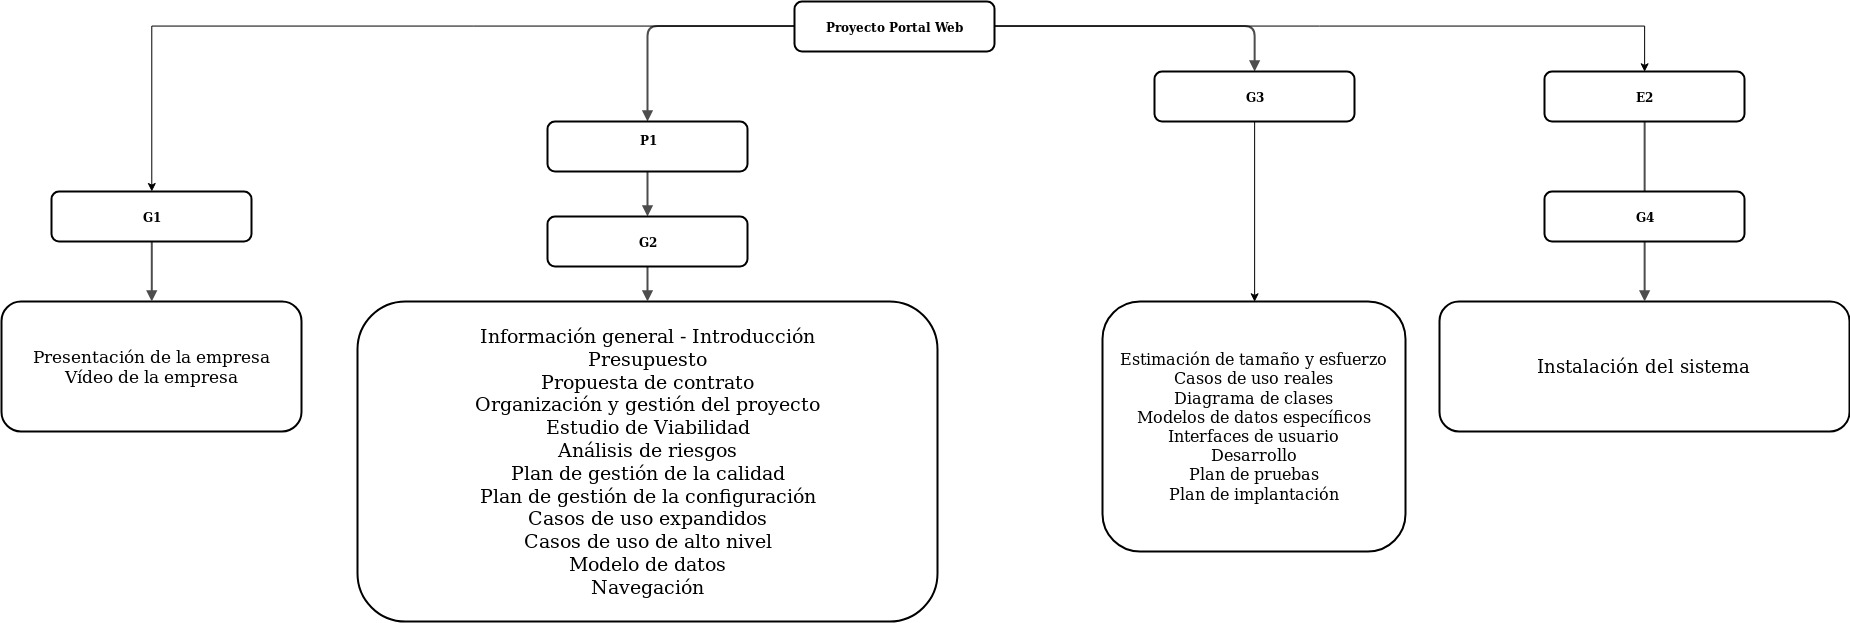
\includegraphics[width=0.8\textwidth]{img/WBS.jpeg}
  \caption{Work Breakdown Structure}
  \label{fig:wbs}
\end{figure}
Figure \ref{fig:wbs} Work Breakdown Structure.


\subsubsection{RBS}
\par A continuación se incluye la captura de MS Project:
\begin{figure}
  \centering
    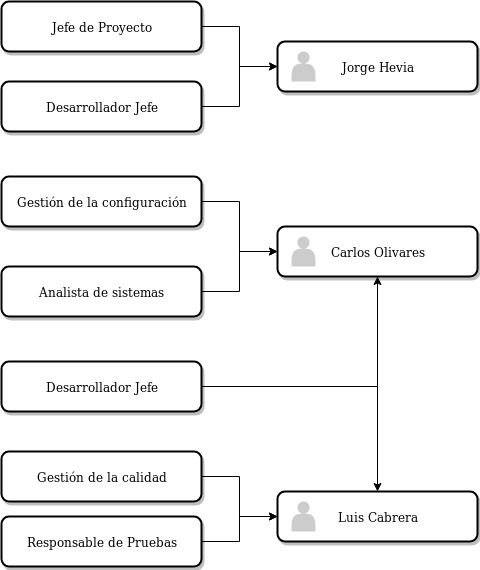
\includegraphics[width=0.8\textwidth]{img/RBS.jpeg}
  \caption{Resources Breakdown Structure}
  \label{fig:rbs}
\end{figure}
Figure \ref{fig:rbs} Resources Breakdown Structure.